\documentclass{article}

\usepackage{graphicx}
\usepackage{tikz}
\usepackage{tikzsymbols}
\usetikzlibrary{calc,patterns,shapes.geometric}
\pagestyle{empty}
\usepackage[margin=0pt]{geometry}
\geometry{papersize={14in,12in}}

\def\centerarc[#1](#2)(#3:#4:#5){\draw[#1] ($(#2)+({#5*cos(#3)},{#5*sin(#3)})$) arc (#3:#4:#5);}

\begin{document}
	\begin{figure}
		\centering
		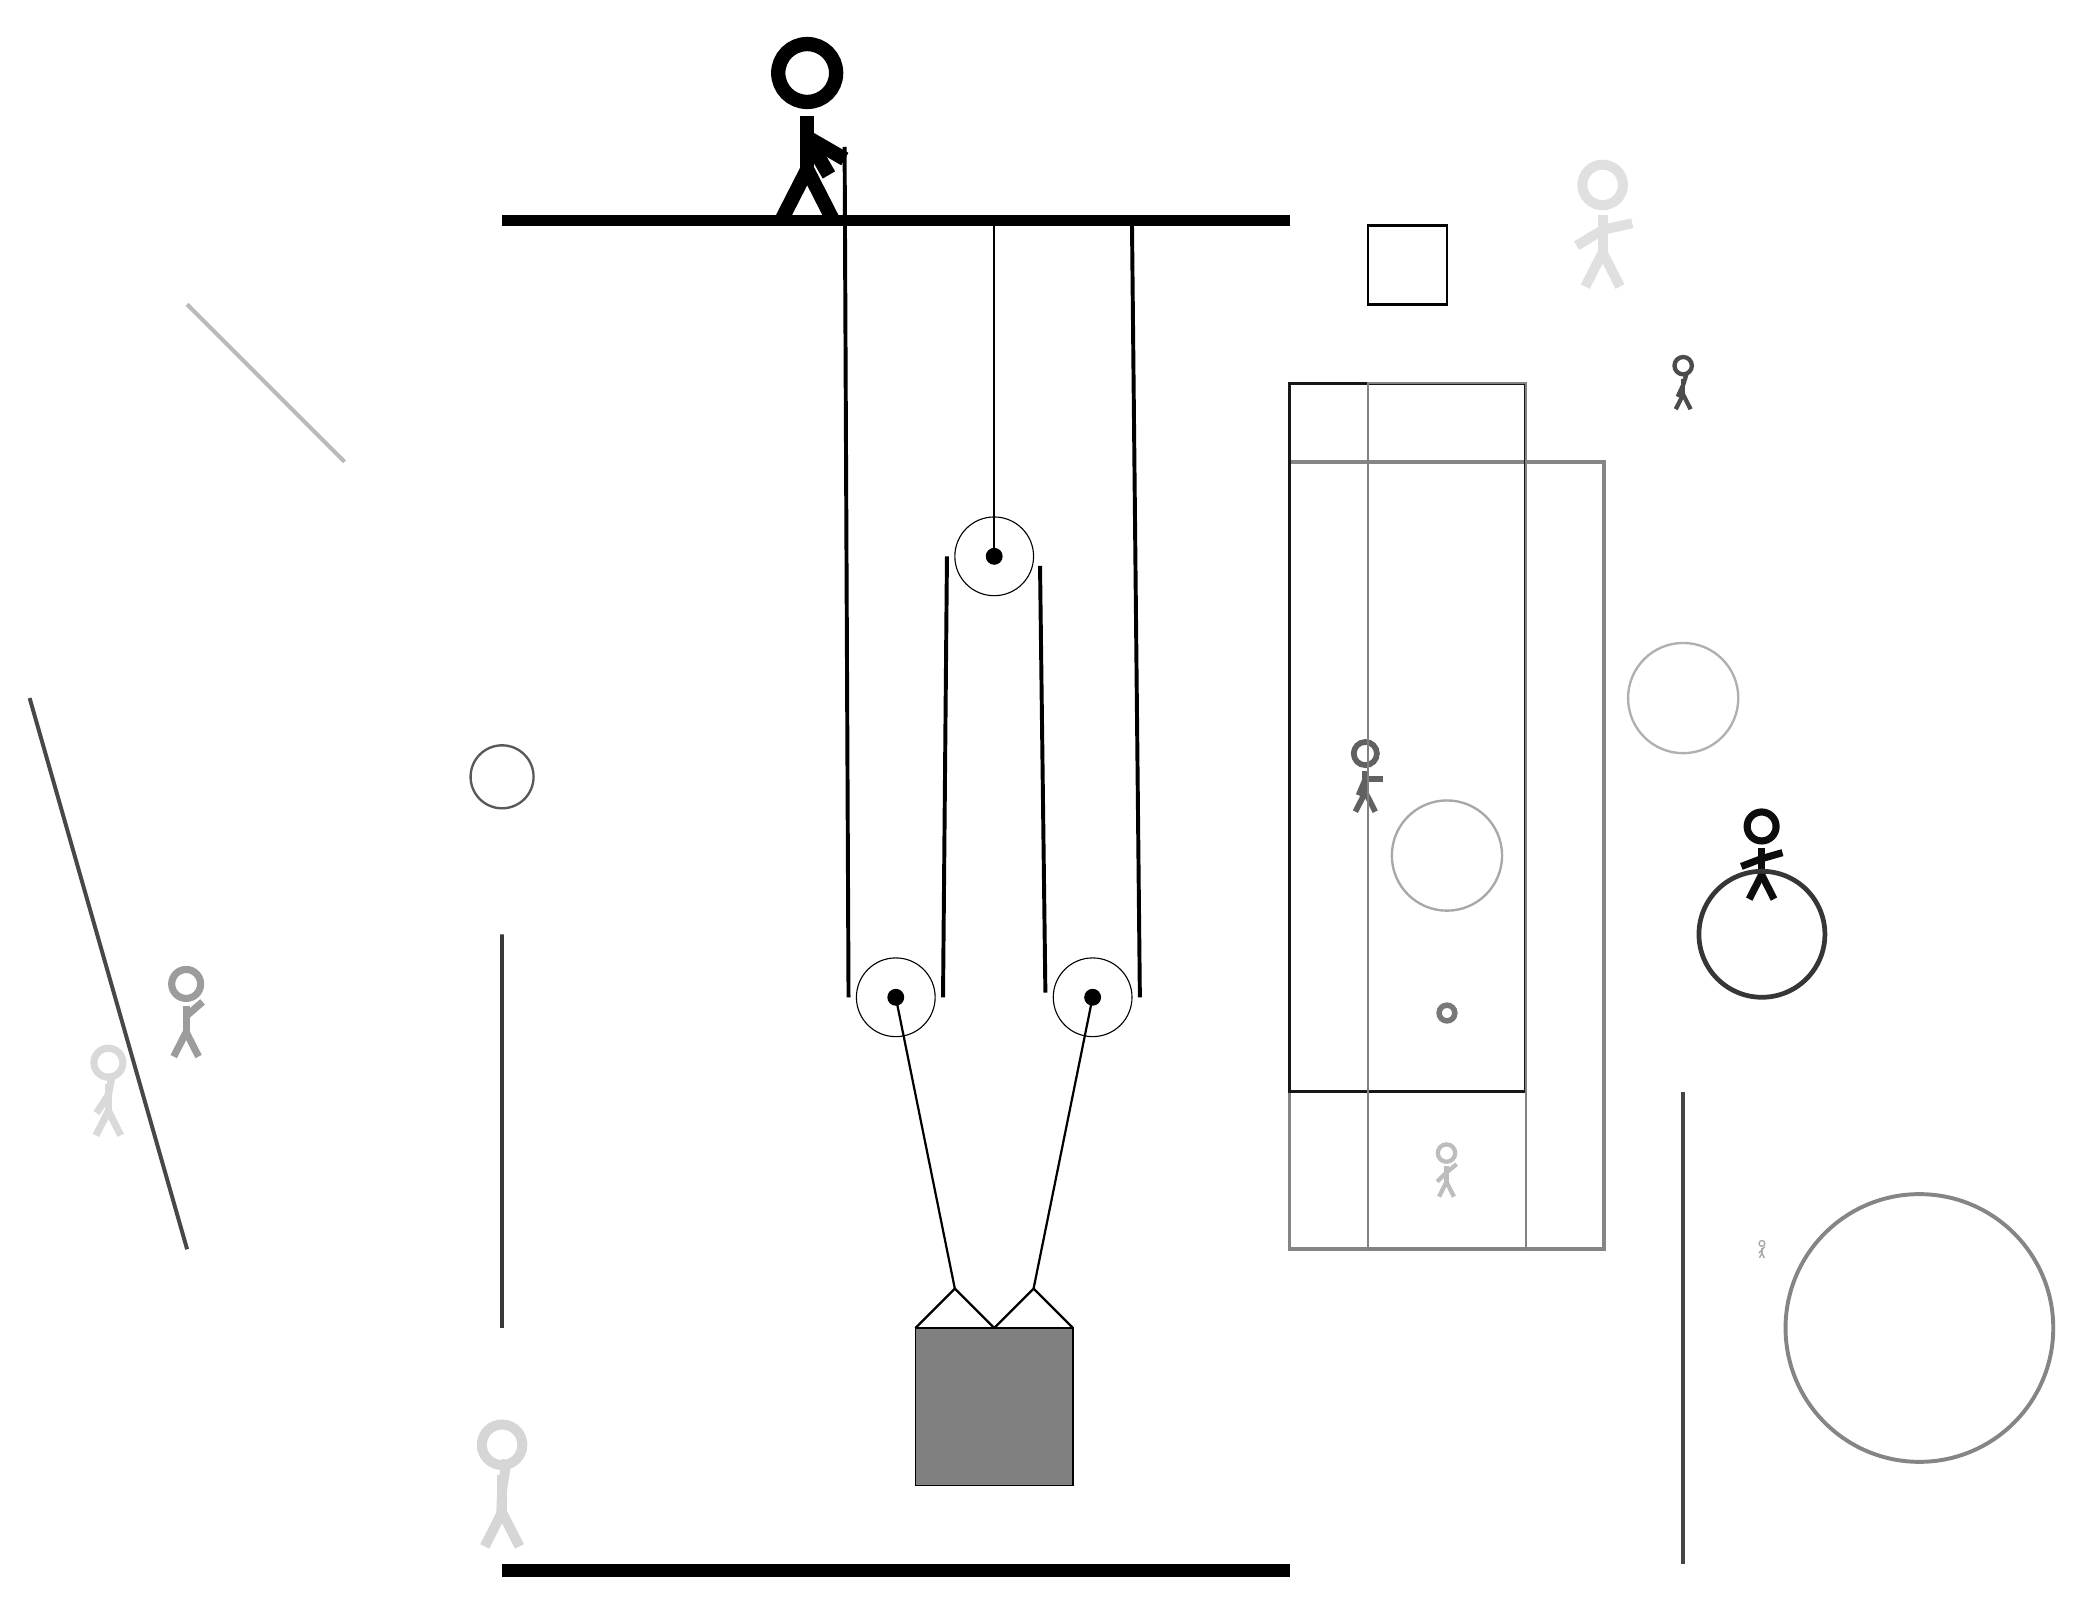
\begin{tikzpicture}
			%%%%% START %%%%%
			
			\draw[fill=black] (-4, 14) rectangle (6, 14.125);
			
			\draw[line width=0.3mm, color=black!99] (7, 14) rectangle (8, 13);
			
			\node[line width=0.2mm, color=black!39] at (-8, 4) {\Strichmaxerl[5][90][41]};
			\draw[line width=0.5mm, color=black!72](-8, 1) -- (-10, 8);
			\node[line width=0.2mm, color=black!95] at (12, 6) {\Strichmaxerl[5][21][16]};
			\node[line width=0.4mm, color=black!15] at (-9, 3) {\Strichmaxerl[5][57][79]};
			\node[line width=0.6mm, color=black!16] at (-4, -2) {\Strichmaxerl[7][88][81]};
			\draw[line width=0.5mm, color=black!48] (6, 1) rectangle (10, 11);
			
			\draw[line width=0.5mm, color=black!78] (-4, 0) rectangle (-4, 5);
			\node[line width=0.3mm, color=black!26] at (8, 2) {\Strichmaxerl[3][45][39]};
			
			\node[line width=0.5mm, color=black!33] at (12, 1) {\Strichmaxerl[1][47][47]};
			\draw [line width=0.3mm, color=black!31](11, 8) circle (0.7);
			\draw[line width=0.5mm, color=black!27](-6, 11) -- (-8, 13);
			\node[line width=0.6mm, color=black!62] at (7, 7) {\Strichmaxerl[4][67][0]};
			\draw[line width=0.4mm, color=black!91] (6, 12) rectangle (9, 3);
			\draw [line width=0.3mm, color=black!34](8, 6) circle (0.7);
			\node[line width=0.7mm, color=black!12] at (10, 14) {\Strichmaxerl[7][31][13]};
			\node[line width=0.5mm, color=black!70] at (11, 12) {\Strichmaxerl[3][65][73]};
			\draw [line width=0.7mm, color=black!53](8, 4) circle (0.1);
			\draw [line width=0.5mm, color=black!48](14, 0) circle (1.7);
			\draw[line width=0.2mm, color=black!49] (7, 1) rectangle (9, 12);
			\draw [line width=0.3mm, color=black!65](-4, 7) circle (0.4);
			
			\draw [line width=0.6mm, color=black!79](12, 5) circle (0.8);
			\draw[line width=0.5mm, color=black!73](11, 3) -- (11, -3);
			
			\draw (1, 4.2) circle (0.5);
			\draw[fill=black] (1, 4.2) circle (0.1);
			
			\draw (2.25, 9.8) circle (0.5);
			\draw[fill=black] (2.25, 9.8) circle (0.1);
			\draw[thick] (2.25, 9.8) -- (2.25, 14);
			
			\draw (3.5, 4.2) circle (0.5);
			\draw[fill=black] (3.5, 4.2) circle (0.1);
			
			\draw[thick] (3.5, 4.2) -- (2.75, 0.5);
			\draw[thick] (1, 4.2) -- (1.75, 0.5);
			\draw[thick]  (1.25, 0) -- (1.75, 0.5) -- (2.25, 0);
			\draw[thick]  (2.25, 0) -- (2.75, 0.5) -- (3.25, 0);
			\draw[fill=black!50] (1.25, 0) rectangle (3.25, -2);
			
			\draw[line width=0.5mm] (0.35, 15) --  (0.4, 4.2);
			\centerarc[line width=0.5mm](1, 4.2)(180:360:0.6);
			\draw[line width=0.5mm] (1.6, 4.2) -- (1.65, 9.8);
			\centerarc[line width=0.5mm](2.25, 9.8)(-20:180:0.6);
			\draw[line width=0.5mm](2.832, 9.68) -- (2.9, 4.26);
			\centerarc[line width=0.5mm](3.5, 4.2)(160:360:0.6);
			\draw[line width=0.5mm](4.1, 4.2) -- (4.0, 14);
			
			\node at (-0.07, 15.2) {\Strichmaxerl[10][120][-30]};
			
			\draw[fill=black] (-4, -3) rectangle (6, -3.15);
			
			%%%%% END %%%%%
		\end{tikzpicture}
	\end{figure}	
\end{document}